\section{Translation, Correction, and Text to Speech}

\setcounter{figure}{0}
\renewcommand{\thefigure}{7.\arabic{figure}}


This chapter is concerned with the final steps of the project. After the dots in the page are detected, now comes the time to start the translation process. Since the model can make mistakes in translating some symbols, a necessary step, text correction, is added. Now that we have a clean text with some, if any, minor mistakes, we can convert it to Speech. The following sections will walk us through these final steps.  

\subsection{Translation}

The translation process in our Braille-to-English text conversion system is a critical component that bridges the gap between the physical Braille script and its digital English text equivalent. This section provides an overview of the methodologies and technologies employed to achieve accurate and efficient translation of scanned Braille images into readable English text. Translating Braille into English text involves recognizing the dot patterns and mapping them to their corresponding characters in the English alphabet. Our system focuses on Grade 1 Braille, which is a direct one-to-one correspondence without contractions, making it a suitable starting point for automated translation. In the following subsections, we will go through the necessary steps of translating a given page written in Braille.

\subsubsection{Data Encoding}

Before beginning the translation process, data was first encoded into sequences of zeros and ones. For example, letter 'A' was encoded into '100000' where '1' indicates the position of a raised dot in the Braille character as follows: 'A': [\braille{1}]. This step is necessary since some Braille characters correspond to two English characters as in the case of the letter 'A' and the number '1', both correspond to the same Braille character of [\braille{1}]. A number is distinguished from a letter by a special character (shown in figure 7.1) that precedes the Braille number. Whenever this special character is encountered inside the loop, we know that the next characters are numbers until a white space is encountered.

\begin{figure}[h]
\centering
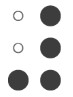
\includegraphics[width=0.15\textwidth]{#.jpg}
\caption{The special character the precedes numbers}
\label{fig:tacotron_model}
\end{figure}

\subsubsection{Image Processing for Braille Detection}

The first step in the translation process is the detection of Braille characters from the scanned images. This involves several stages of image processing to ensure that the Braille dots are accurately identified. These steps have been covered in chapter 5.

\subsubsection{Deep Learning for Character Recognition}

Once the Braille dots are detected and organized, the next step is to recognize these patterns as specific Braille characters. Our system employs a deep learning model to achieve high accuracy in this recognition process. The process of model training has been covered in chapter 6.

\subsubsection{Mapping Braille to English Text}

The recognized Braille characters are then mapped to their corresponding English text equivalents. This step involves:

\begin{enumerate}
    \item \textbf{Character Mapping}: Each detected Braille pattern is mapped to a predefined English character based on the Braille alphabet. This is a straightforward one-to-one mapping in the case of Grade 1 Braille. After the characters have been recognized, they are then saved in a list in the same order in which they appeared in the Braille page.
    \item \textbf{Handling Punctuation and Special Characters}: Special consideration is given to punctuation marks and other non-alphabetic characters to ensure they are accurately represented in the translated text. For example, numbers are preceded with a special character to indicate that the character after it is a number. The same goes for punctuation marks. Punctuation marks representations in Braille are shown in figure 7.2.
\end{enumerate}

\begin{figure}[h]
\centering
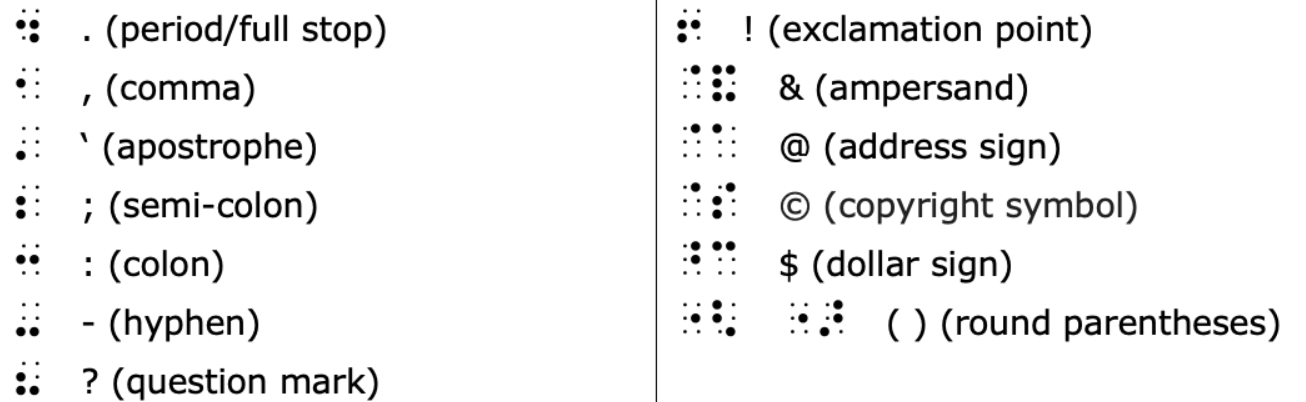
\includegraphics[width=1\textwidth]{punctuation.png}
\caption{Punctuation marks in Braille}
\label{fig:tacotron_model}
\end{figure}

\subsubsection{Integration and Output}

The final stage of the translation process is integrating all the components to produce a coherent English text output:

\begin{enumerate}
    \item \textbf{Text Assembly}: After saving the recognized characters in a list, the characters are assembled into words and sentences by looping through the list, preserving the original structure and formatting of the Braille content.
    \item \textbf{Output Formatting}: The translated text is formatted for readability by, for example, removing any extra white spaces and formatting the paragraphs as they appeared in the original text.
\end{enumerate}


\subsection{Text Correction}
After translation, there were some words with spelling mistakes, the most common error being character substitution due to incorrect symbol recognition. Correcting these mistakes requires contextual text correction. Through research, we identified a package called 'contextualSpellCheck' which performs this task, and a pre-trained model known as 'T5-large-spell' model.

\subsubsection{Python's ‘contextualSpellCheck’ Package}
\begin{enumerate}
    \item \textbf{How it works:}
 \begin{figure}
\centering
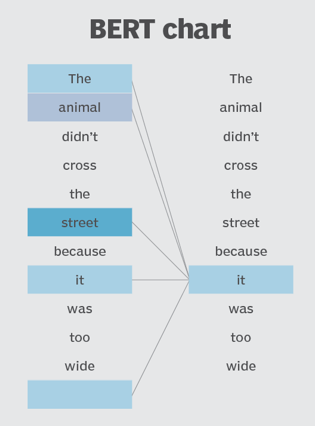
\includegraphics[]{bert.PNG}
\caption{Example on BERT self-attention-mechanism}
\label{fig:bert}
\end{figure}
    The 'contextualSpellCheck' package relies on BERT (Bidirectional Encoder Representations from Transformers) for contextual text correction. BERT, introduced by Google in 2018, is a pre-trained natural language processing (NLP) model based on the Transformer architecture. Transformers are neural networks designed for sequence-to-sequence tasks, where one Transformer (encoder) processes the input sequence and another Transformer (decoder) generates the output sequence. The encoder converts the input sequence into abstract representations, and the decoder generates the output sequence by attending to these representations, trained using supervised learning techniques. 
    
    BERT's bidirectional training approach allows it to consider context from both the left and right sides of a given word in a sentence, enhancing its understanding of natural language. BERT models are trained using large repositories of specialized, labeled data, involving manual data labeling by linguists. Initially, BERT was pretrained using a collection of unlabeled text from sources like the entire English Wikipedia and the Brown Corpus, totaling about a million words. BERT continues to learn through unsupervised learning from unlabeled text and improves with use in practical applications such as Google search. 
    
    The model also relies on self-attention mechanisms, which capture and understand relationships among words in a sentence. This is significant because a word's meaning can change as a sentence develops. BERT reads bidirectionally, accounting for the effect of all other words in a sentence on the focus word and eliminating left-to-right momentum that biases words towards a certain meaning. This allows BERT to accurately predict words in context, enhancing its ability to understand and process natural language.
    
    Figure \ref{fig:bert} explains how the self-attention mechanism works: BERT determines which prior word in the sentence the word 'it' refers to, using the self-attention mechanism to weigh the options. The word with the highest calculated score is deemed the correct association. In this example, 'it' refers to 'animal', not 'street'. If this phrase were a search query, the results would reflect this subtler, more precise understanding that BERT reached.
    
    Additionally, BERT uses Next Sentence Prediction (NSP) as a training technique. NSP teaches BERT to predict whether a certain sentence follows another by providing both correctly paired and wrongly paired sentence pairs. Over time, BERT gets better at predicting the next sentence accurately.


    \item \textbf{Testing:}
    While using this package, we found that it sometimes replaces names with pronouns. We attempted to address this issue by comparing the erroneous sentences with their correct counterparts, but this approach proved ineffective. Another issue is that it alters some words in the context unnecessarily. Consequently, we decided not to use this package for our project and began searching for an alternative.
\clearpage
\begin{figure}
\centering
\subfloat[]{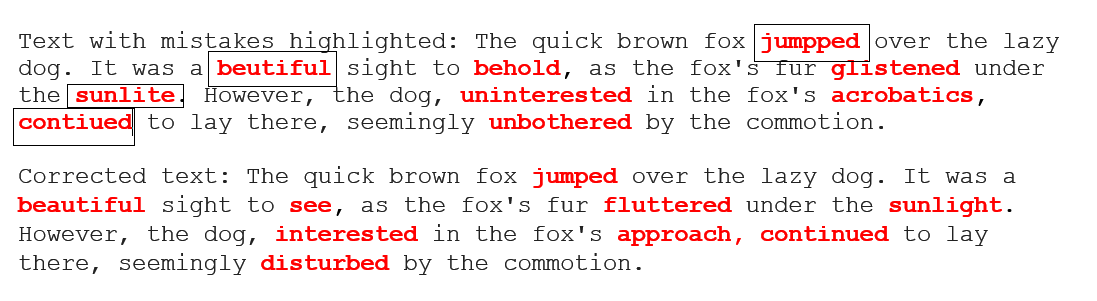
\includegraphics[width=\linewidth]{spellcheck1.PNG}}\hfill
\subfloat[]{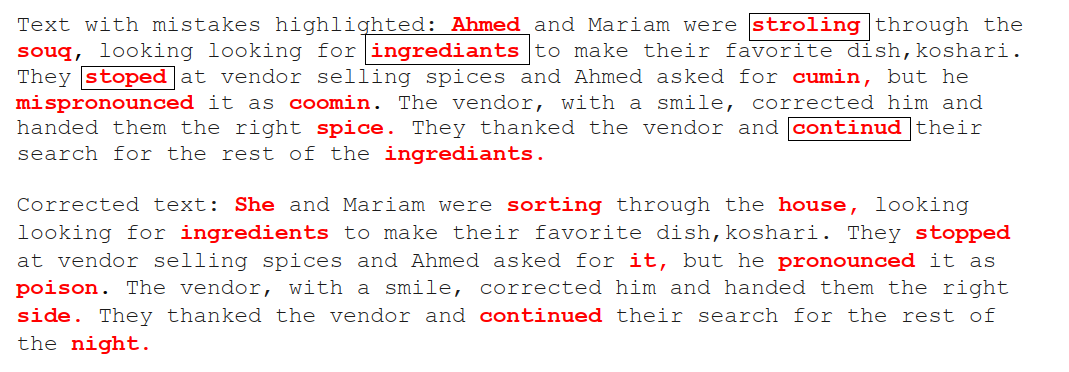
\includegraphics[width=\linewidth]{spellcheck2.PNG}}
\caption{Some Problems of the packet}
\label{fig:spell} 
\end{figure}

    Figure \ref{fig:spell}(a) illustrates that the packet corrected all the misspelled words, highlighted by squares, while also substituting some words with alternatives it deemed more suitable.

    Figure \ref{fig:spell}(b) demonstrates that the packet corrected all the misspelled words, indicated by squares, but concurrently replaced some of the names with pronouns and substituted place names or food names with their descriptions.
\end{enumerate}


\subsubsection{The Pre-trained ‘T5-large-spell’ Model}
\begin{enumerate}
    \item \textbf{How it works:}
    The 'T5-large-spell' model refers to a variant of the T5 (Text-To-Text Transfer Transformer) model architecture that has been specifically fine-tuned for the task of spell checking. Text-To-Text Transfer Transformer (T5) is a powerful model architecture, developed by Google AI, that revolutionizes natural language processing (NLP) tasks by treating them all as text-to-text problems. T5 is based on the Transformer architecture, which uses self-attention mechanisms, as explained previously, to capture relationships between words in a sequence. This allows the model to understand the context and meaning of words in a sentence. T5 treats every task as a text-to-text transformation, meaning both input and output are in text format, making the model’s architecture simpler and more consistent.
    
    The T5-large model is pre-trained on a vast amount of text data, which includes a diverse range of sources such as books, articles, websites, and more. This ensures that the model learns from a wide variety of linguistic contexts and styles. During pre-training, a significant part of the input text is randomly masked (replaced with a special token, [MASK]), and the model is tasked with predicting the original words that were masked. The objective is to train the model to understand the relationships between words in a sentence or sequence by leveraging the context provided by the surrounding words. This process encourages the model to learn robust representations of words and their meanings based on their context within sentences and documents. By predicting masked tokens, the T5-large model learns to generate representations (embeddings) for each word or subword that capture its meaning in different contexts. These contextual representations allow the model to understand subtle nuances in language, such as word sense disambiguation (choosing the correct meaning of a word based on context) and syntactic structures.
    \item \textbf{Testing:}
    During our testing, we observed that the model requires a significant amount of time to correct sentences. Despite our efforts, fine-tuning the model to reduce processing time was unsuccessful. Additionally, we encountered an issue where the model would add words to incomplete input sentences (those not ending with a full stop) in an attempt to complete them.
    To address this, we implemented a simple workaround: adding a full stop at the end of each sentence before input and removing it after correction. Another solution involved comparing the word count of the input and output sentences and removing any extra words from the output.
    It is also worth noting that the model’s accuracy is 83\%. However, our specific use case involves small paragraphs with a limited number of misspelled words, so this accuracy level is acceptable for our needs.
\clearpage
\begin{figure}
\centering
\subfloat[]{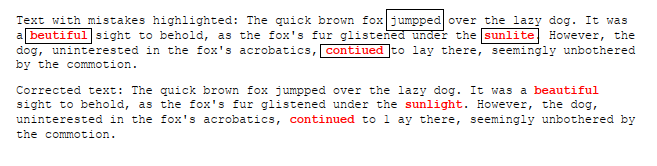
\includegraphics[width=\linewidth]{T5_1.PNG}}\hfill
\subfloat[]{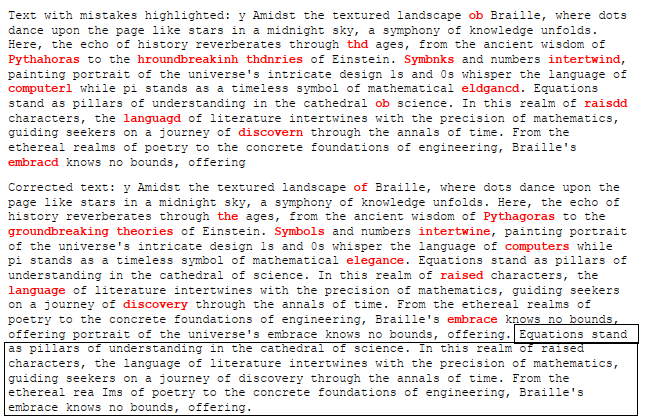
\includegraphics[width=\linewidth]{T5_3.PNG}}
\caption{Some Problems of the T5 model}
\label{fig:t5} 
\end{figure}

Figure \ref{fig:t5}(a) shows that not all the incorrect words were corrected; there was a word which was not corrected.

Figure \ref{fig:t5} (b)demonstrates that when the sentence was incomplete, there were some redundant words (highlighted by square) that were added. 

    
\end{enumerate}

\subsection{Text to Speech Conversion}
\paragraph{In this project, we explored several text-to-speech (TTS) synthesis models before selecting the Tacotron model for our final implementation. Initially, we experimented with FastPitch, Glow TTS, Tacotron 2, Overflow, DeepVoice, and WaveNet models. Each model offered unique advantages and posed specific challenges, which ultimately guided our decision to utilize Tacotron.}


\subsubsection{DeepVoice}

DeepVoice is a TTS model designed to closely mimic the human speech production process. It uses a pipeline architecture with distinct modules for text analysis, phoneme prediction, duration prediction, frequency prediction, and waveform synthesis. The modularity of DeepVoice allows for fine-grained control over each component of the TTS process.

\begin{figure}[h]
\centering
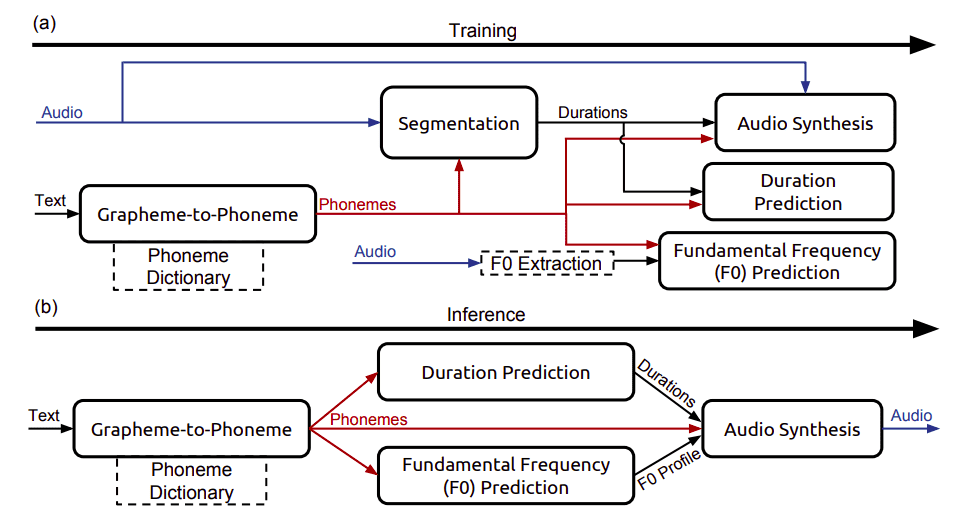
\includegraphics[width=0.8\textwidth]{deepvoice.png}
\caption{DeepVoice model architecture, showing the pipeline from text analysis to waveform synthesis.}
\label{fig:deepvoice_model}
\end{figure}

While this modular approach provides flexibility, it also introduces complexity and requires extensive hand-tuning of each module. Moreover, the separation of tasks can lead to suboptimal interactions between components, affecting the overall speech quality.



\subsubsection{WaveNet}

WaveNet is a generative model that produces raw audio waveforms directly from text input. It leverages dilated causal convolutions to model long-range temporal dependencies, resulting in high-quality, natural-sounding speech. The model operates at the sample level, generating one audio sample at a time. Despite its superior audio quality, WaveNet's computational requirements are significantly higher due to its sample-level generation approach. This makes real-time inference challenging and computationally expensive. The trade-off between quality and computational cost was a key consideration in our evaluation.


\begin{figure}[h]
\centering
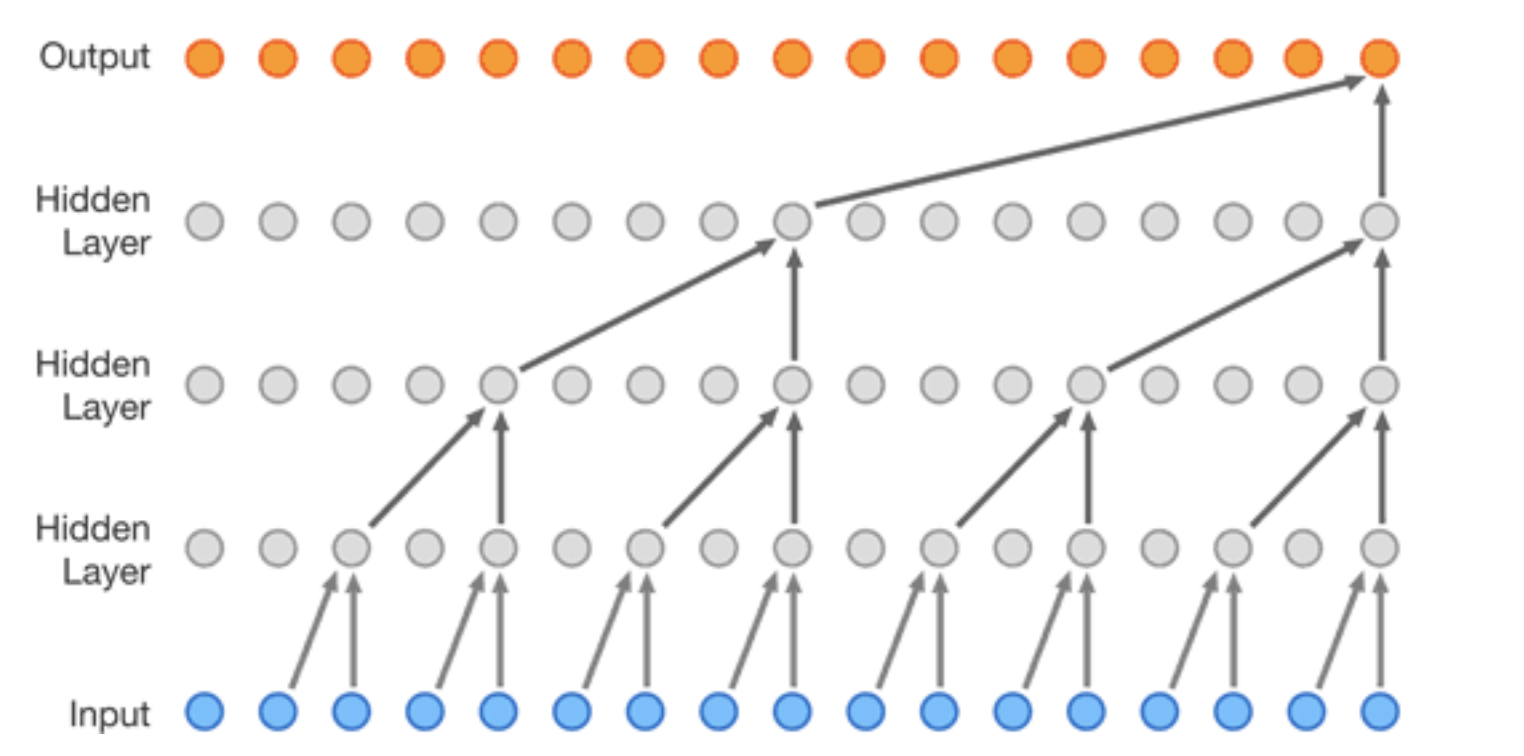
\includegraphics[width=0.8\textwidth]{dilated convolution.png}
\caption{Illustration of dilated causal convolutions used in WaveNet to capture long-range dependencies.}
\label{fig:dilated_convolutions}
\end{figure}

\subsubsection{Tacotron}

We ultimately selected the Tacotron model for its balance between complexity and performance. Tacotron, as described by Wang et al. (2017), is an end-to-end speech synthesis system that directly converts text into speech. The model integrates feature extraction, sequence learning, and waveform generation into a single framework, streamlining the TTS pipeline.

\begin{figure}[h]
\centering
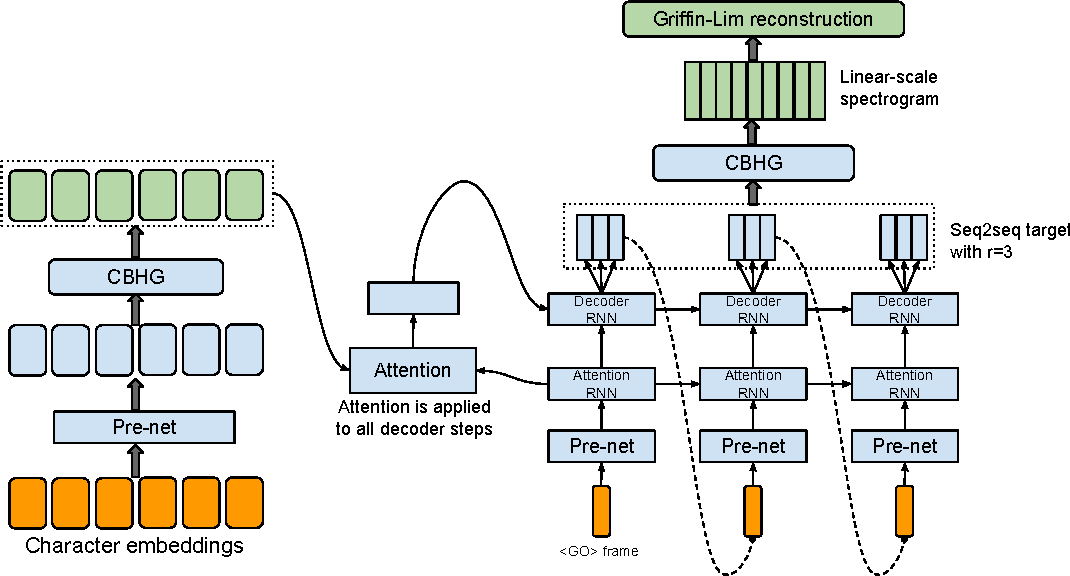
\includegraphics[width=0.8\textwidth]{tacotron.png}
\caption{Tacotron model architecture as described by Wang et al. (2017).}
\label{fig:tacotron_model}
\end{figure}

\paragraph{Encoder}\mbox{}


The encoder converts the input text into a sequence of feature vectors. It first embeds each character into a continuous representation. These embeddings are then processed through a stack of convolutional layers, which capture local dependencies and create a robust representation. The output is then passed through a bidirectional Long Short-Term Memory (LSTM) network, capturing long-range dependencies in both forward and backward directions. Additionally, the encoder employs a CBHG (1-D Convolution Bank, Highway Network, and Bidirectional GRU) network to further refine the encoded features.

\paragraph{Attention-Based Decoder}\mbox{}


The attention-based decoder generates mel-spectrogram frames from the encoded feature vectors. This module uses an LSTM-based network combined with an attention mechanism to dynamically focus on different parts of the encoded sequence. This ensures that the generated speech aligns with the input text. The decoder iteratively predicts multiple non-overlapping mel-spectrogram frames at each time step, which improves the convergence speed and alignment stability. Similar to the encoder, the decoder also includes a CBHG network to enhance the quality of the predicted mel-spectrograms.

\paragraph{CBHG Post-Processing Network}\mbox{}


The CBHG module (1-D Convolution Bank, Highway Network, and Bidirectional GRU) refines the generated mel-spectrogram frames into linear spectrograms, which are then converted into waveforms using a vocoder. The CBHG module includes:

\begin{itemize}
    \item \textbf{1-D Convolution Bank}: Applies multiple convolutional filters of different widths to capture a variety of local patterns in the input sequence.
    \item \textbf{Highway Network}: Facilitates information flow and enables training of deeper networks by allowing for both direct and transformed paths of information.
    \item \textbf{Bidirectional GRU}: Captures sequential dependencies in both forward and backward directions, refining the feature representation for final spectrogram generation.
\end{itemize}

\begin{figure}[h]
\centering
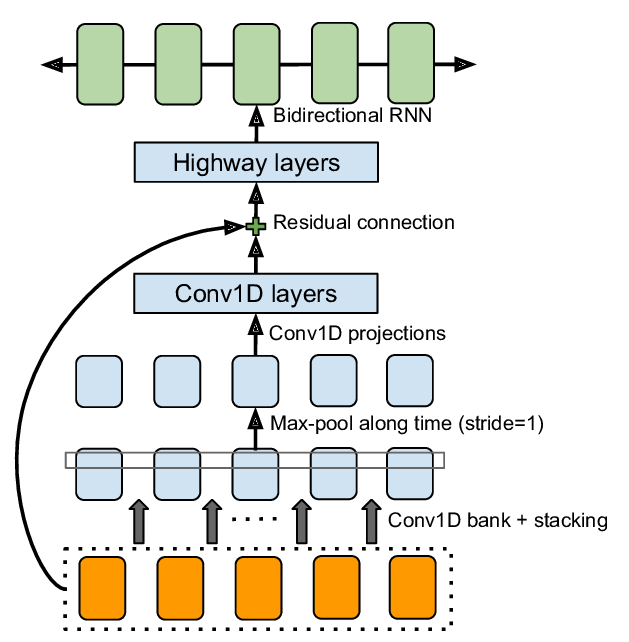
\includegraphics[width=0.5\textwidth]{cbhg.png}
\caption{CBHG module architecture used in the Tacotron model for post-processing.}
\label{fig:cbhg_module}
\end{figure}

\paragraph{Griffin-Lim Algorithm}\mbox{}

The Griffin-Lim Algorithm is a method for reconstructing a signal from its spectrogram, primarily used in audio processing. This iterative algorithm refines an initial estimate of the signal by minimizing the difference between the magnitude of the spectrogram of the estimated signal and the target spectrogram.

The process starts with an initial guess of the signal. The magnitude of its spectrogram is then replaced with the target spectrogram while keeping the phase unchanged. The updated signal is then reconstructed using the inverse Short-Time Fourier Transform (STFT). This process is repeated iteratively until convergence, yielding a signal whose spectrogram matches the target spectrogram as closely as possible.

To understand this better, we need a brief explanation of the Fourier Transform. The Fourier Transform is a mathematical operation that transforms a signal from its original domain (often time or space) into the frequency domain. The result is a representation of the signal as a sum of sinusoidal components, each with a specific frequency, amplitude, and phase. In audio processing, the Short-Time Fourier Transform (STFT) is typically used, which breaks the signal into small overlapping segments and applies the Fourier Transform to each segment, producing a time-frequency representation known as a spectrogram.

The Griffin-Lim Algorithm leverages this time-frequency representation to iteratively refine the phase information of the signal, resulting in a high-quality reconstruction from the magnitude spectrogram alone.

\begin{figure}[h]
\centering
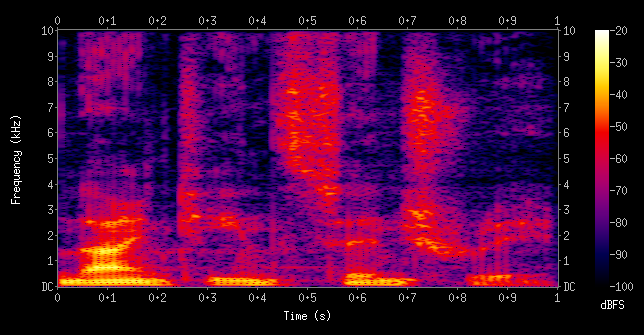
\includegraphics[width=0.5\textwidth]{spectrogram.png}
\caption{Example Spectrogram.}
\label{fig:cbhg_module}
\end{figure}

\subsubsection{Tacotron 2}

Tacotron 2 improves upon the original Tacotron model by integrating WaveNet as a neural vocoder, resulting in higher quality speech synthesis. Tacotron 2 utilizes an attention-based sequence-to-sequence model to map text to mel-spectrograms, followed by WaveNet to generate the waveform. However, we chose Tacotron over Tacotron 2 for several reasons:

\begin{itemize}
    \item \textbf{Simplicity and Integration}: The original Tacotron model integrates feature extraction, sequence learning, and waveform generation into a single framework, simplifying implementation and maintenance compared to Tacotron 2, which introduces additional complexity through WaveNet integration.
    
    \item \textbf{Computational Efficiency}: Tacotron 2, while providing higher audio quality, is computationally expensive due to its use of WaveNet. In contrast, the original Tacotron is more computationally efficient, making it suitable for environments with limited resources or real-time applications.
    
    \item \textbf{Implementation and Resource Constraints}: Given our project's constraints, including limited computational resources and a need for straightforward implementation, the original Tacotron model was more feasible than Tacotron 2.
    
    \item \textbf{Quality vs. Complexity Trade-off}: While Tacotron 2 offers superior audio quality with WaveNet, the additional complexity and computational demands may not justify the quality improvement in our specific use case.
    
    \item \textbf{Familiarity and Expertise}: Our team had prior experience with the original Tacotron model, which facilitated faster development and easier integration into our existing workflow.
    
    \item \textbf{Griffin-Lim Algorithm}: The original Tacotron model's use of the Griffin-Lim algorithm for waveform reconstruction is simpler to implement and understand compared to the neural vocoder approach in Tacotron 2.

    
\end{itemize}

\subsubsection{Other Pre-trained Models}

\begin{itemize}
    \item \textbf{FastPitch} 
    is a TTS model that focuses on fast and high-quality speech synthesis by predicting pitch contours alongside the mel-spectrograms, resulting in more expressive and natural-sounding speech.
    
    \item \textbf{Glow TTS}
     is based on generative flow models, which are designed to produce high-quality speech with better control over the generated outputs. It uses normalizing flows to transform simple distributions into more complex ones that model the target speech data.

    \item \textbf{Overflow}
    is a TTS model designed for efficient and high-quality speech synthesis, focusing on reducing latency and computational cost while maintaining high-quality outputs.
\end{itemize}


\subsubsection{Conclusion}

After evaluating the performance and requirements of all the previously mentioned models, we found that Tacotron provided the optimal balance of quality, simplicity, and computational efficiency for our text-to-speech synthesis needs. The end-to-end nature of the Tacotron model allowed us to streamline the TTS pipeline, achieving high-quality, natural-sounding speech with less complexity and lower computational cost.


